\addbibresource{reference.bib}

\chapter{Handler}\label{chap:handler}

V této kapitole bude čtenář podrobně seznámen s handlerem - komponentou pro distribuované řízení detektorů. Jak již bylo zmíněno v kapitole \ref{chap:arch}, handler je komponenta zajišťující komunikaci a vyčítání dat z detektorů (viz obr. \ref{fig:handler:overview}) skrze poskytnuté implementace komunikačního a datového interface.
  
Handler implementuje \textit{Spring framework} (viz \ref{chap:arch:technologie:spring}), aby mohl poskytovat \texttt{REST API} pro management detektorů a pro poskytování stavových informací o své instanci. Handler dále poskytuje jednoduché webové rozhraní s přehledem připojených detektorů.

Na obrázku \ref{fig:handler:overview} je znázorněn příklad instance handleru z pohledu vstupu (pět přiřazených detektorů) a pohledu výstupu (poskytované \texttt{REST API} a webové rozhraní.)

\begin{figure}[bh]
	\begin{center}
		\vspace*{1cm}
		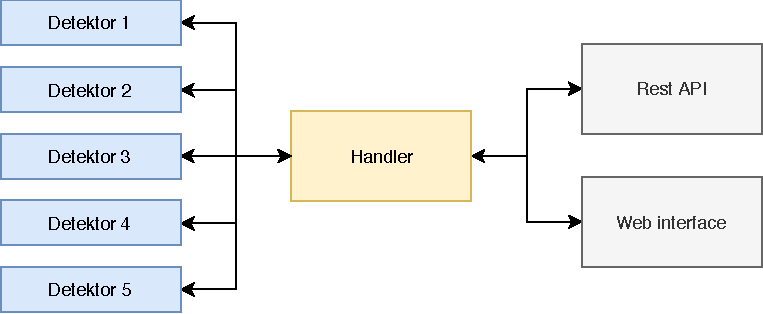
\includegraphics[width=14cm]{figures/handler_overview.pdf}
		\caption{Pixnet - handler: příklad instance handleru s pěti připojenými detektory, poskytujícího REST API pro své řízení a webové uživatelské rozhraní s přehledem připojených detektorů.}
		\label{fig:handler:overview}
	\end{center}
\end{figure}

\newpage

%********************************************************************************
% Vrstvy softwarové architektury
%********************************************************************************
\section{Vrstvy softwarové architektury}\label{chap:handler:architecture}
Tato podkapitola je věnována softwarové architektuře handleru. Budou zde představeny jednotlivé její vrstvy, tj. od vrstvy pro komunikaci s detektorem, management detektorů, Spring implementaci, až po výstupní vrstvu poskytující \texttt{REST API} a webové rozhraní - viz obr. \ref{fig:handler:arch}. Vybrané vrstvy budou popsány detailněji v dalších podkapitolách.

\begin{figure}[th]
	\begin{center}
		\vspace*{0.4cm}
		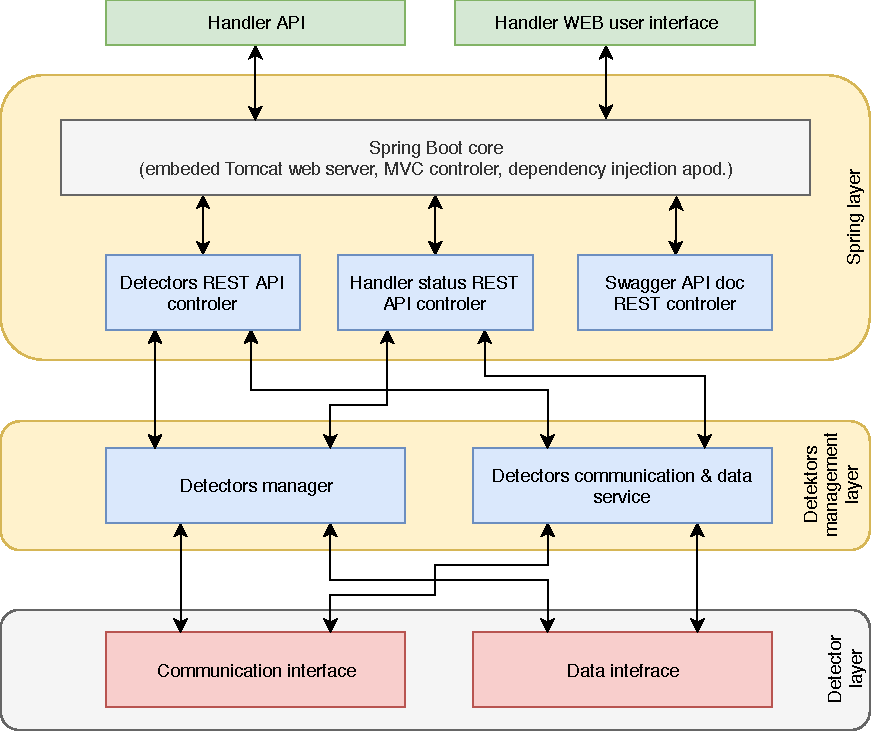
\includegraphics[width=14cm]{figures/handler_architecture.pdf}
		\caption{Pixnet - handler: softwarová architektura s vrstvami pro (i) rozhraní detektoru (\textit{Detector layer}), (ii) management detektorů (\textit{Detectors management layer}),(iii) Spring vrstvu (\textit{Spring layer}) a (iv) výstupní vrstvou pro \texttt{REST API} a webové uživatelské rozhraní.}
		\label{fig:handler:arch}
	\end{center}
\end{figure}

\subsection{Detektorová vrstva}\label{chap:handler:detector_layer}
Detektorová vrstva se skládá ze dvou částí - externě poskytnuté implementace komunikačního a datového interface. Tyto tzv. moduly jsou zavedené až za běhu programu pomocí vyšších vrstev systému.

\subsubsection{Zavádění modulů}
Každý modul, obsahující implementaci komunikačního, nebo datového interface, musí pro své zavedení do systému splňovat následující kritéria:

\begin{itemize}
	\item Musí být zkompilován do Java archívu (\texttt{*.jar}) - současná verze implementace podporuje pouze moduly vyvinuté v jazyce Java (resp. také v jazyce Kotlin, zkompilovaného do Java \textit{bytecode}), v dalších verzích je plánováno přidání podpory pro \texttt{C++} a \texttt{Python}.
	\item Při vývoji modulu musí být použit datový model, který je součástí poskytovaných knihoven.
	\item Modul musí obsahovat implementaci jednoho z již zmíněních rozhraní. Navíc, celý název implementující třídy (vč. tzv. \texttt{package}) musí být uveden jako atribut s názvem \texttt{PluginImplClass} v manifestu \texttt{jar} archívu, viz zdrojový kód \ref{src:handler:manifest}.
\end{itemize}

\begin{minted}[
    frame=single,
	linenos,
	breaklines
  ]{html}
  Manifest-Version: 1.0
  PluginImplClass: cz.ctu.ieap.pixnet.handler.detector_communication_katherine.CommImpl  
\end{minted}
\begin{code}[h!]
\caption{Příklad obsahu souboru \texttt{MANIFEST.MF}, obsaženého v \texttt{jar} archívu modulu.}
\label{src:handler:manifest}
\end{code}


\subsubsection{Komunikační rozhraní}
Zdrojový kód \ref{src:handler:comm_intf} obsahuje interface, který komunikační modul detektoru musí implementovat.

Prvních pět metod (tj. řádek 3 až 7) má čistě informativní charakter a jejich implementace má čistě informativní charakter pro operátora systému.

Na řádcích 8 a 9 je setter a getter pro konfiguraci detektoru. Konfigurace je detektoru předána jako \texttt{String}\footnote{Datový typ obsahující textový řetězec} (setter) a musí být do něj serializovatelná (getter). Systém ale s konfigurací detektoru neumí pracovat (kromě komunikačního modulu detektoru, resp. implementace komunikačního interface), tudíž jejíž syntax není vynucována a její podoba je čistě v kompetenci poskytovatele komunikačního modulu. Avšak je doporučeno, aby zvolený formát byl strojově i lidsky čitelný, z důvodu jeho snazší editace\footnote{V dalších fázích implementace systému je plánováno přidání podpory editace konfigurace v rámci webového uživatelského rozhraní mastera.}. Takový formát může být na příklad \texttt{JSON}\footnote{Z angl. \textit{JavaScript Object Notation} (JavaScriptový objektový zápis).}, nebo \texttt{YAML}\footnoteUrl{http://yaml.org/}, který je použit pro serializace konfigurace komunikačního modulu Katherine (viz \todo přidat ref.).

\begin{minted}[
    frame=single,
	linenos,
	breaklines
  ]{kotlin}
interface DetectorComm {

  fun getDetectorType(): DetectorType
  fun getReadoutName(): String
  fun getSensorsCount(): Int
  fun getDetectorWidth(): Int
  fun getDetectorHeight(): Int
  fun setDetectorConfig(config: String)
  fun getDetectorConfig(): String?
  fun getSupportedValueCommands(): List<AbstractValueCommand>
  fun getSupportedExecutionCommands(): List<AbstractExecutionCommand>
  fun getAcceptedFilesKeys(): List<String>
  fun getDataFrameQueue(): BlockingQueue<AbstractDataFrame>
  
  fun isConnected(): Boolean
  fun connect(): Boolean
  fun disconnect(): Boolean
  
  fun executeSetValueCommand(commandID: Int, payload: ValuePayload)
  fun executeGetValueCommand(commandID: Int): ValuePayload
  fun executeExecutionCommand(commandID: Int, input: Map<String, ValuePayload>): Map<String,  ValuePayload>
  fun uploadFile(fileKey: String, file: ByteArray)
  fun setCallback(callback: Callback)
  
  interface Callback {
    val classLoader: ClassLoader?
  }

}
\end{minted}
\begin{code}[h!]
\caption{Komunikační interface detektoru, napsané v jazyce Kotlin (viz \ref{chap:arch:technologie:kotlin})).}
\label{src:handler:comm_intf}
\end{code}

Pro získání seznamu podporovaných \textit{value commands} (tj. příkazů pro operace s jednotlivými hodnotami detektoru) slouží metoda \texttt{getSupportedValueCommands()}, viz řádek 10. \texttt{AbstractValueCommand} má v modelu poskytované knihovny dvě implementace:
\begin{enumerate}[label=(\roman*)]
	\item \texttt{ValueCommand} obsahuje atributy pro daného příkazu, tj.:
	\begin{itemize}
		\item \textbf{id} - celočíselný unikátní identifikátor daného příkazu,
		\item \textbf{name} - název příkazu, resp. manipulované hodnoty detektoru,
		\item \textbf{valueUnit} - jednotka veličiny manipulované hodnoty detektoru (může nabývat hodnot z \textit{Enum} třídy \texttt{ValueUnit} poskytovaného modelu, např. \texttt{ValueUnit.VOLT} apod.),
		\item \textbf{accessType} - modifikátor přístupu manipulované hodnoty, který může nabývat těchto hodnot:
		\begin{description}
			\item[\texttt{SETTER}] pro takové hodnoty, které je možné pouze nastavovat,
			\item[\texttt{GETTER}] pro takové hodnoty, které je možné pouze číst a
			\item[\texttt{SETTER\_AND\_GETTER}] pro hodnoty, které je možné nastavovat i číst.
		\end{description}
		\item \textbf{valueModel} - datový model hodnoty daného příkazu, který definuje datový typ veličiny (podporovány jsou \texttt{Boolean}, \texttt{String}, \texttt{Integer}, \texttt{Long}, \texttt{Float} a \texttt{Double}) a omezení rozsahu hodnot. Model může být diskrétní (tzn. hodnota může nabývat jen nějaké z předem definovaných hodnot), nebo spojitý (hodnota může nabývat jakékoliv hodnoty ze zadaného intervalu).
	\end{itemize}
	Viz zdrojový kód \ref{src:handler:value_command} pro příklad definice \textit{ValueCommand} pro \textit{bias} (prahové napětí detektoru).

	\item \texttt{ValueCommandGroup} je třída pro seskupování příkazů podobného významu (např. \texttt{DAC} hodnoty detektoru) a obsahuje název skupiny příkazů a seznam jednotlivých\\\texttt{ValueCommands}.
\end{enumerate}

\begin{minted}[
    frame=single,
	linenos,
	breaklines
  ]{java}
valueCommands.add(ValueCommand(
    42, // id
    "Bias", // name
    ValueUnit.VOLT, // valueUnit
    SETTER_AND_GETTER, // accessType
    FloatValueModel(-300f, 300f) // valueModel
))
\end{minted}
\begin{code}[h!]
\caption{Příklad definice \textit{ValueCommand} detektoru pro příkaz s názvem \textit{"Bias"}, id 42, jednotkou Volt, modifikátorem přístupu \textit{Setter \& Getter} a reálným modelem hodnot, omezeným intervalem $<-300,300>$.}
\label{src:handler:value_command}
\end{code}

Pro vykonání \texttt{ValueCommand} je třeba implementovat metody \texttt{executeSetValueCommand()} a \texttt{executeGetValueCommand()}, viz řádky 19 a 20 komunikačního interface (zdrojový kód \ref{src:handler:comm_intf}). První metoda slouží pro nastavení hodnot a akceptuje ID příkazu a \texttt{valuePayload}, který obsahuje hodnotu jednoho ze šesti podporovaných datových typů, a je možné jej vykonat pouze pro příkazy, které mají \texttt{accessType}, umožňující zápis hodnot. Druhá metoda slouží pro čtení hodnot, jako vstupní parametr má ID příkazu a její návratový typ je \texttt{ValuePayload}, obsahující hodnotu čteného parametru.

Dalším typem příkazů je získání seznamu podporovaných \texttt{ExecutionCommands} (viz 11. řádek komunikačního interface \ref{src:handler:comm_intf}). Od \texttt{ValueCommands} se liší tím, že vstup a výstup není omezen stejnou veličinou (resp. jejím modelem hodnot) a ani jejich množstvím. Tento přístup tedy umožňuje definovat příkazy, které mají 0 až m vstupních hodnot a 0 až n výstupních hodnot. Obdobně jako \texttt{AbstractValueCommand}, i \texttt{AbstractExecutionCommands} má v poskytované knihovně dvě implementace:
\begin{enumerate}[label=(\roman*)]
	\item \texttt{ExecutionCommand} je definován obdobně jako \texttt{ValueCommand} - má své ID, jméno, ale také obsahuje seznamy rozšířených modelů hodnot - jeden vstupní a jeden výstupní. Rozšířený model hodnot obsahuje již zmíněný \texttt{valueModel}, dále pak jméno hodnoty, její ID (textový řetězec) a \texttt{valueUnit}.
	
	Zdrojový kód \ref{src:handler:execution_command} obsahuje příklad s \texttt{ExecutionCommand} pro nastavení akvizičního módu detektoru. Z příkladu je patrné, že příkaz akceptuje právě dvě vstupní hodnoty (akviziční mód a \textit{FastVCO} přepínač) a že žádné hodnoty nevrací.
	
	\item \texttt{ExecutionCommandGroup} je obdobou třídy \texttt{ValueCommandGroup} pro \texttt{ExecutionCommand}. Obsahuje název skupiny příkazů a jejich seznam.
\end{enumerate}

\begin{minted}[
    frame=single,
	linenos,
	breaklines
  ]{java}
executionCommands.add(ExecutionCommand(
  KatherineExecutionCommands.SET_ACQ_MODE.internalID, // ID (Int)
  "Set acquisition mode", // name
  // model vstupných hodnot
  arrayOf(
    ValueModelVerbose(
      "Acquisition mode", // název hodnoty
      ValueId.acq_mode.name, // ID hodnoty (String)
	  // celočíselný diskrétní model hodnot
	  IntValueModel(mapOf(
        Pair("ToA & ToT", 0),
        Pair("ToA", 1),
        Pair("Event & iToT", 2)
      )),
      ValueUnit.DIMENSIONLESS // jednotka hodnoty
    ), 
    ValueModelVerbose(
      "Fast vco enabled",
      ValueId.fast_vco_en.name,
      BooleanValueModel(mapOf(
        Pair("Enable", true),
        Pair("Disable", false)
      )),
      ValueUnit.DIMENSIONLESS
	)
  ),
  null // model výstupních hodnot
))
\end{minted}
\begin{code}[h!]
\caption{Příklad definice \textit{ExecutionCommand} pro nastavování akvizičního módu detektoru s vyčítacím rozhraním \textit{Katherine} (viz \ref{chap:detectors:readouts:katherine}). Z příkladu je patrné, že vstupní model je tvořen dvěma hodnotami a výstupní model je prázdný.}
\label{src:handler:execution_command}
\end{code}

Pro vykonání \texttt{ExecutionCommand} slouží metoda \texttt{executeExecutionCommand()}, viz řádek 21 komunikačního interface (zdrojový kód \ref{src:handler:comm_intf}). Metoda akceptuje ID příkazu a mapu (tzn. seznam párů klíč - hodnota) jednotlivých hodnot. Klíčem v mapě je ID parametru a hodnota je již výše zmíněný \texttt{ValuePayload}, obsahující hodnotu parametru. Výstupem volání metody je pak mapa výstupních parametrů příkazu.

Pro přípojení detektoru, odpojení detektoru a zjišťování stavu připojení slouží metody \texttt{connect()}, \texttt{disconnect()} a \texttt{isConnected()} (viz řádky 15 až 17 zdrojového kódu \ref{src:handler:comm_intf}). Aby bylo možné provést jakoukoliv operaci interagující s detektorem (tj. vykonávání příkazů a nahrávání souborů) je nutné, aby byl detektor připojen, resp. metoda \texttt{isConnected()} musí vracet \texttt{true}.

Do detektorů rodiny \textit{Medipix} je třeba před jejich použitím nahrát konfiguraci jednotlivých pixelů detektoru. Konfigurace je pole bytů, kde nastavení jednoho pixelu je serializováno do jednoho bytu. Z tohoto důvodu je třeba přidat podporu pro nahrávání velkých binárních objektů (tzv. \texttt{LOB}\footnote{Z angl. Large Object.}).
Pro nahrávání souborů do detektoru slouží příkaz \texttt{uploadFile()} (viz řádek 22 zdrojového kódu \ref{src:handler:comm_intf}), který akceptuje ID souboru a jeho binární reprezentaci. Pro poskytnutí seznamu podporovaných souborů, resp. jejich ID, je třeba implementovat metodu \texttt{getAcceptedFilesKeys()} (viz řádek 12 zdrojového kódu \ref{src:handler:comm_intf}).

V kapitole \ref{chap:arch:sw:detector} již byl popsán tok měřených dat v handleru, resp. od komunikačního k datovému modulu. Přenos dat je realizován asynchronní blokující frontou (viz obr. \ref{fig:handler:data_queue}), tj. frontou ke které může asynchronně přistupovat více vláken současně a zároveň čtení z fonty je implementováno jako blokující operace (tzn. že zablokuje čtecí vlákno, než bude ve frontě nějaký element v vyčtení). Jelikož komunikační modul je zodpovědný za vytvoření instance fronty, tak její implementace je zcela v kompetenci poskytovatele komunikačního modulu. Jedinou podmínkou je, aby fronta implementovala interface \texttt{BlockingQueue}\footnote{Z \textit{Java Collections Framework}.}. V další části textu (viz \ref{chap:katherine}) bude čtenář seznámen s implementací komunikačního modulu s implementací fronty pomocí \texttt{LinkedBlockingQueue}\footnote{Implementace \texttt{BlockingQueue} pomocí spojového seznamu. V této frontě jsou elementy řazení pomocí FIFO (first-in-first-out). Fronty založené na spojové struktuře umožňují (ve srovnání s frontami založenými na dynamickém poly) vyšší datový tok, zejména pro vícevláknové aplikace.}.
\begin{figure}[h]
	\begin{center}
		\vspace*{0.5cm}
		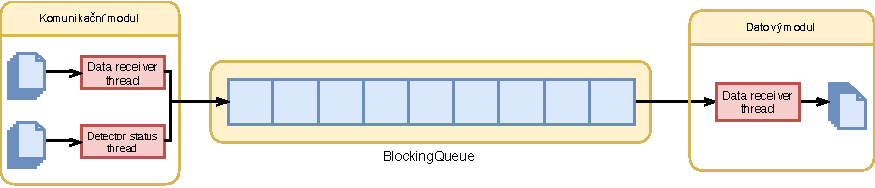
\includegraphics[width=14.5cm]{figures/handler_data_queue.pdf}
		\caption{Asynchronní blokující fronta naměřených dat s příkladem produkujících vláken v komunikačním modulu a přijímacím vláknu v datovém modulu.}
		\label{fig:handler:data_queue}
	\end{center}
\end{figure}

Poslední metodou komunikačního interface je metoda \texttt{setCallback()} (viz 23. řádek komunikačního interface (zdrojový kód \ref{src:handler:comm_intf})). Tato metoda je handlerem zavolána bezprostředně po inicializaci modulu a modul si může uložit referenci na předaný \texttt{callback} (instanci interface \texttt{Callback} z komunikačního interface). \texttt{Callback} slouží například k získání Java \texttt{ClassLoader}, kterým byl modul načten (používá se například pro parsing konfigurace).

\subsubsection{Datové rozhraní}


\subsection{Vrstva managementu detektorů}\label{chap:handler:detectors_layer}


\subsection{Spring vrstva}\label{chap:handler:spring}